\chapter{Problematic}

\thispagestyle{empty}

The rise of Distributed Denial of Service (DDoS) attacks poses a significant threat to network security, making it crucial to develop effective detection mechanisms. In the context of machine learning, the challenge lies in accurately identifying DDoS attacks from normal network traffic data. 

Detecting DDoS attacks presents several challenges due to the dynamic and evolving nature of these attacks. Traditional detection methods often fall short in accurately identifying DDoS attacks, leading to increased risk and potential downtime for organizations. There is a critical need for an effective and efficient DDoS detection solution that can adapt to the changing nature of attacks. Machine learning offers a promising approach to DDoS detection, thanks to its ability to analyze large volumes of data and identify complex patterns that may indicate an ongoing attack. 

In this project, our objective is to develop a web application that provides users with an interface to upload their Packet Capture (PCAP) files. The application will then process these files and present the results in a tabular format, indicating whether the traffic is classified as NORMAL or as a DDoS attack.


\section{What is a DDoS attack ?}

A distributed denial-of-service (DDoS) attack is analogous to a group of people crowding the entry door of a shop, making it hard for legitimate customers to enter, thus disrupting trade and losing the business money. 

It is a malicious attempt to disrupt the normal traffic of a targeted server, service or network by overwhelming the target or its surrounding infrastructure with a flood of Internet traffic.
\begin{figure}[h]
	\centering
	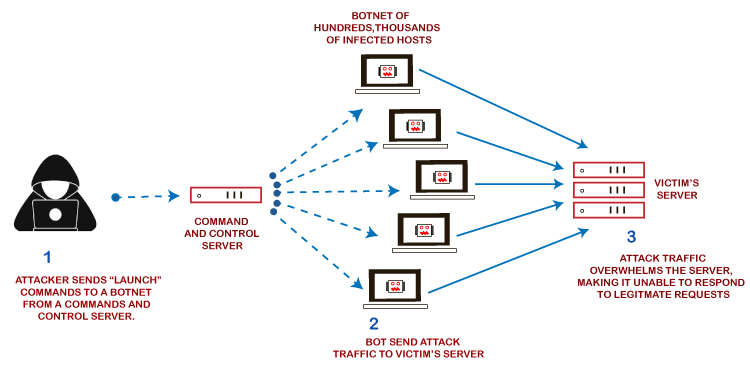
\includegraphics[width=0.9\textwidth]{./assets/images/what-is-ddos-attack.png}
	\caption{DDoS attack}
\end{figure}

\pagebreak
\section{Structure of a PCAP file}
\textbf{A PCAP file} is a binary file format that stores network traffic data. It captures packets in a structured manner, preserving the details of each communication unit traversing a network. These files are instrumental for network administrators, analysts, and cybersecurity professionals in diagnosing network issues, monitoring activities, and investigating security incidents.


The PCAP's file structure is defined by three fundamental components : the Global Header (PCAP Header), the Packet Headers, and the Packet Data.
\begin{figure}[h]
	\centering
	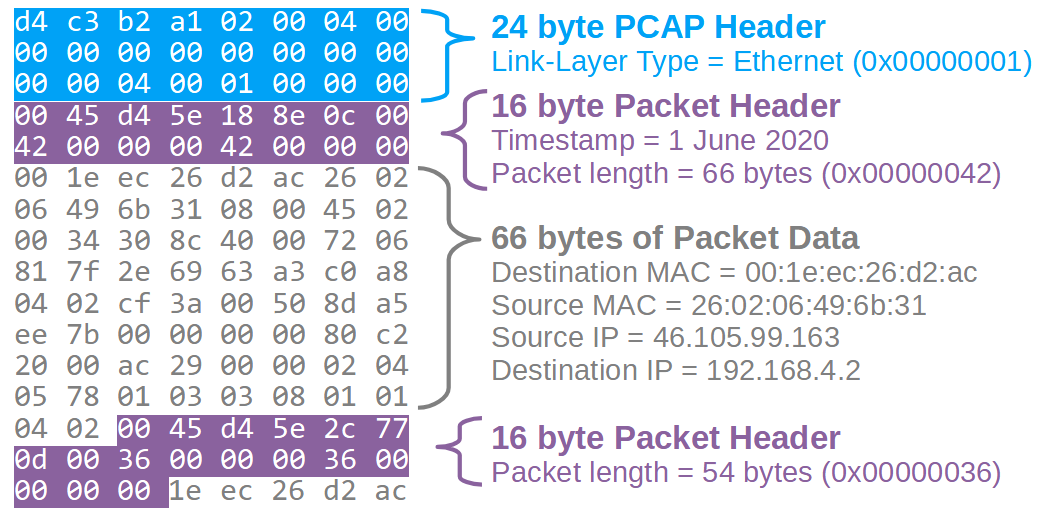
\includegraphics[width=0.9\textwidth]{./assets/images/PCAP-header-hex_1040x520.png}
	\caption{PCAP file structure}
\end{figure}

%\section{Random Forest Classifier}

%\subsection{Decision Trees}
%A Decision Tree is a white box type of \textbf{supervised learning} algorithm that is used for both \textbf{classification} and \textbf{regression} tasks. They learn a series of hierarchical \textbf{`if/else`} questions to classify data or predict outcomes.
%\begin{figure}[h]
%	\centering
%	\includegraphics[width=1\textwidth]{./assets/images/g}
%	\caption{Decision Trees example}
%\end{figure} 








